\section{Introduction to train a Neural Network} %Jianhong / b-j8497 / Jul 10
\subsection{PyTorch Basics} % Author: Jonathan Siegel
In this section, we will introduce PyTorch \footnote{\url{https://pytorch.org}} which is an open source machine learning framework that accelerates the path from research prototyping to production deployment. 

The basic class underlying pytorch is the tensor class. This class simply represents an array of numeric values (usually floats or doubles) and behaves very similar to the corresponding class in numpy.
\begin{python}
import torch
import numpy as np

# We can initialize a pytorch tensor from a python list.
x = torch.tensor([[1,2],[3,4]])
print('x is', x)

# Or from a numpy array.
y = torch.tensor(np.array([[1,2],[3,4]]))
print('y is', y)

# We can also initialize a zeroed tensor.
a = torch.zeros([2,2])
b = torch.zeros([3,3], dtype=torch.int32)

# Note that the default type of such a tensor is a 32-bit float.
print('Type of a:', a.dtype)
print('Type of b:', b.dtype)
\end{python}
The output will be
\begin{python}
x is tensor([[1, 2],
        [3, 4]])
y is tensor([[1, 2],
        [3, 4]])
Type of a: torch.float32
Type of b: torch.int32
\end{python}
Arithmetic operations on PyTorch tensors work as one would expect.
\begin{python}
z = 2*x
print(z)

z = y - z
print(z)

z = torch.matmul(x,y)
print(z)

# etc. see the documentation for more details.
\end{python}
It gives
\begin{python}
tensor([[2, 4],
        [6, 8]])
tensor([[-1, -2],
        [-3, -4]])
tensor([[ 7, 10],
        [15, 22]])
\end{python}


At this point, there isn't much difference between Pytorch and Numpy. What distinguishes Pytorch and makes it useful for Deep Learning is the automatic differentiation supported by Pytorch (essentially, Pytorch can automatically apply the chain rule to calculate derivatives). We illustrate this below with a simple example.
\begin{python}
# In this example we calculate the derivative of (x.y)^2 w.r.t x.

# In order to calculate the gradient with respect to a tensor,
# we must set the requires_grad flag to True.
x = torch.tensor([1.0, 0.0], requires_grad=True)
y = torch.tensor([1.0, 1.0])

# By default, requires_grad is set to False if possible.
print('y.requires_grad:', y.requires_grad)

z = torch.dot(x, y)

# Because z depends on x, which requires a gradient, z.requires_grad
# is automatically set to true. This is done because the gradient of z
# is needed to calculate the gradient of x.
print('z.requires_grad:', z.requires_grad)

out = z * z

# Calculate the derivative of out w.r.t. x. Automatically applies
# the chain rule as needed.
grad = torch.autograd.grad(outputs=out, inputs=x)
print(grad)
\end{python}
The output will be
\begin{python}
y.requires_grad: False
z.requires_grad: True
(tensor([2., 2.]),)
\end{python}

Using what we have so far, we can automatically differentiate polynomials (since they are just compositions of elementary arithmetic operations). But what about more complicated differentiable functions? We can deal with those by subclassing torch.autograd.Function as we show in the next example.
\begin{python}
# We illustrate this by implementing the pointwise ReLU function
# (which is of course already implemented in Pytorch, but this
# process can be used to define more complex custom functions as well).

# We subclass torch.autograd.Function to define new functions
class MyReLU(torch.autograd.Function):
  
  # The forward method applies the function to the input argument.
  # The ctx argument can be used to cache information for the subsequent
  # gradient computation. You can cache an object using using the 
  # ctx.save_for_backward method.
  @staticmethod
  def forward(ctx, input):
    # The input is needed later to calculate the gradient.
    ctx.save_for_backward(input)
    return input.clamp(min=0)
  
  # The backward method calculates the gradient of the input, given that
  # the gradient of the output is the output_grad argument.
  def backward(ctx, output_grad):
    # Recover the original input from ctx.
    input, = ctx.saved_tensors
    grad_input = output_grad.clone()
    # Zero out the output gradient where the input is negative to obtain
    # the input gradient.
    grad_input[input < 0] = 0
    return grad_input
    
# Apply the new function to a tensor.
print(MyReLU.apply(x - 0.5))
    
# Calculating derivatives utilizes the backward method.
z = torch.mul(MyReLU.apply(x - 0.5), y)
# In this case z is not a scalar, so we must provide the derivatives
# of the outputs. What is actually computed is the gradient of 
# z dot output_grad with respect to x.
output_grad = torch.ones([2])
print(torch.autograd.grad(outputs=z, inputs=x, grad_outputs = output_grad))
\end{python}
\begin{python}
tensor([0.5000, 0.0000], grad_fn=<MyReLUBackward>)
(tensor([1., 0.]),)
\end{python}
We have seen how to define a custom function. Luckily, we won't have to do this much work very often. As we will see, many common functions in machine learning have already been implemented for us.

Next we introduce the Variable class in torch.autograd. This class used to be necessary for autograd, but since regular tensors now allow for automatic differentiation, it is basically just a wrapper around the tensor class which introduces a few additional methods, most notably the .backward() method.
\begin{python}
from torch.autograd import Variable

# Variables can be copy constructed from tensors. When constructed, we can 
# also specify whether the gradient is required or not.
x = Variable(x, requires_grad=True)
y = Variable(y, requires_grad=False)

# All functions which can be applied to tensors can also be applied to 
# Variables. In the code below, z will be a Variable since x and y are.
# In general, if at least one input is a Variable, then the output will be as
# well.
z = torch.mul(MyReLU.apply(x - 0.5), y)

# Notably, we can now call .backward() from z_variable, which will compute 
# the gradient with respect to z for all tensors it depends on (if their
# requires_grad field is True). Note that since z isn't a scalar, we still
# need to pass the gradients of each of its components.
z.backward(gradient=output_grad)

# The resulting gradients are stored in the .grad field of the corresponding
# tensors. The gradients are only calculated if requires_grad = True.
print('x gradient:', x.grad)
print('y gradient:', y.grad)
\end{python}
\begin{python}
x gradient: tensor([1., 0.])
y gradient: None
\end{python}
Since Variables contain all of the functionality as tensors, but contain additional methods (especially the very useful .backward() method) as well, we recommend using Variables for all non-constant quantities in your code. We illustrate some of the additional behaviors of the .backward() function below.
\begin{python}
# A very important note is that gradients are accumulated, i.e. added to
# whatever is already stored in the .grad field.
z = torch.mul(MyReLU.apply(x - 0.5), y)
z.backward(gradient=output_grad)
print('x.grad has now been doubled:', x.grad)

# In order to avoid this, we must first clear the gradient of x. Note also
# that in the above example we need to recompute z in terms of x and y 
# in order to recompute the gradient. We can avoid this by setting 
# retain_graph = True
x.grad.data.zero_()
z = torch.mul(MyReLU.apply(x - 0.5), y)
z.backward(gradient=output_grad, retain_graph=True)
print('x gradient:', x.grad)

# Since we set retain_graph=True during the last backward call, we can 
# recompute the gradients without recalculating z. This feature is not
# commonly used and considered bad practice, though.
x.grad.data.zero_()
z.backward(gradient=output_grad)
print('x gradient:', x.grad)
\end{python}
\begin{python}
x.grad has now been doubled: tensor([2., 0.])
x gradient: tensor([1., 0.])
x gradient: tensor([1., 0.])
\end{python}

\subsection{Building Neural Networks} % Author: Jonathan Siegel
Building and training neural networks directly using Pytorch Variables and automatic differentiation would be very cumbersome. Luckily, Pytorch provides built-in functionality which makes it much easier to build and train neural networks. In this section, we will describe how to use this functionality to build (i.e. define) a network.

The most important library for building neural networks is the torch.nn library. This library allows us to build neural networks by concatenating different types of layers.
\begin{python}
import torch.nn as nn

# Here we define a sample neural network. The class defining our
# network should inherit from nn.Module.
class Net(nn.Module):
  def __init__(self):
    super(Net, self).__init__()
    # Here we define the layers of the network.
    # The nn.Sequential method constructs a model by concatenating
    # the layers which are input to it.
    self.apply = nn.Sequential( # Sequentially apply a
        nn.Linear(10,20),       # Linear function R^10 -> R^20
        nn.ReLU(),              # Pointwise ReLU
        nn.Linear(20,20),       # Linear function R^20 -> R^20
        nn.ReLU(),              # Pointwise ReLU
        nn.Linear(20,10))       # Linear function R^20 -> R^10

  # The following method must be overloaded. It specifies how to
  # evaluate the model given an input x.
  def forward(self, x):
    return self.apply(x) # In our instance we simply pass x through
                         # the previously defined layers. This could
                         # potentially contains something more complex.
\end{python}
Implementing a Logistic Regression
We will now consider the problem of implementing a logistic regression (trained using stochastic gradient descent) using Pytorch. We will test this model on the MNIST handwritten data imageset.
\begin{python}
import torch
import torchvision
import torchvision.transforms as transforms
import matplotlib.pyplot as plt
import numpy as np

# Transforms images from [0,255] to [0,1] range.
transform = transforms.Compose(
    [transforms.ToTensor(),
     transforms.Normalize(mean=[0], std=[1])])

# Load the set of training images.
trainset = torchvision.datasets.MNIST(root='./data', train=True, download=True, transform=transform)
trainloader = torch.utils.data.DataLoader(trainset, batch_size=4, shuffle=True, num_workers=2)

# Load the set of test images.
testset = torchvision.datasets.MNIST(root='./data', train=False, download=True, transform=transform)
testloader = torch.utils.data.DataLoader(testset, batch_size=4, shuffle=False, num_workers=2)

# Let's plot some of the images to see what we're dealing with.
def plot_images(imgs):
  for i in range(imgs.size()[0]):
    npimg = imgs.numpy()[i,0,:,:]
    plt.imshow(npimg, cmap='gray')
    plt.ion()
    plt.show()
    plt.pause(.05)

data = iter(testloader)
images, labels = data.next()
print(labels)
plot_images(images)
\end{python}
Now that we've loaded our dataset, let's build the logistic regression model. In the language of deep learning, the logistic regression is the same as a neural network with no hidden layers trained with a cross entropy loss (exercise: work this out yourself!).
\begin{python}
# This library contains a lot of useful classes for constructing 
# neural networks and other machine learning models.
import torch.nn as nn

# This model simply takes an input of dimension 784 and multiplies it 
# by a 784x10 matrix of parameters.
class LogisticRegression(nn.Module):
  def __init__(self):
    super(LogisticRegression, self).__init__()
    self.dense_linear = nn.Sequential(
      nn.Linear(28 * 28, 10))

  def forward(self, x):
    x = x.view(-1,28*28)
    x = self.dense_linear(x)
    return x
  
# Construct an instance of the model.
model = LogisticRegression()
\end{python}

Now we need to fit the parameters of this logistic regression model (the 784x10 matrix). We do this by defining a loss function (the cross entropy) and using the stochastic gradient descent optimization algorithm. Luckily, both of these have already been implemented for you in Pytorch!
\begin{python}
# This library contains implementations of a number of useful optimization algorithms.
import torch.optim as optim

# The cross entropy loss is already implemented in Pytorch.
criterion = nn.CrossEntropyLoss()

# The stochastic gradient descent algorithm with a step size of 0.1.
optimizer = optim.SGD(model.parameters(), lr=0.1)

# Write a loop to train the model using the given optimizer and loss functions.
for i in range(20):
  for data in trainloader:
    # extract the images and labels.
    inputs, labels = data
    
    # This must be called to zero out the accumulated gradients.
    optimizer.zero_grad()
    
    # Calculate the predictions made based on the model.
    outputs = model(inputs)
    
    # Evaluate the loss function based on the model predictions.
    loss = criterion(outputs, labels)
    
    # Calculate the gradient of the parameters with respect to the loss.
    loss.backward()
    
    # Take a optimization step.
    optimizer.step()
    
  print('Completed epoch %d' % i)
print('Completed training')
\end{python}
Now that we've trained our model, we will test its accuracy on the test dataset.
\begin{python}
# Calculate the total number of test samples and the number of correctly 
# classified test samples
correct = 0
total = 0
for data in testloader:
  images, labels = data
  outputs = model(images)
  # Take the most likely label as the predicted label.
  _, predicted = torch.max(outputs.data, 1)
  total += labels.size(0)
  correct += (predicted == labels).sum()

print('Out of %d samples, the model correctly classified %d' % (total, correct))
\end{python}

\subsection{Datasets}
In this section, we will talk about how to train a neural network. According to the course in the morning, there are a lot of pictures in a dataset, so, at the beginning, we will introduce some famous and popular datasets. 
\begin{itemize}
\item {\bf MNIST}\footnote{\url{http://yann.lecun.com/exdb/mnist/}} contains 60,000 pictures of the ten handwritten digits from 0 to 9. The size of each picture is $28\times 28$ pixels. There are 60,000 pictures for training and 10,000 for testing.
\begin{figure}
\centering
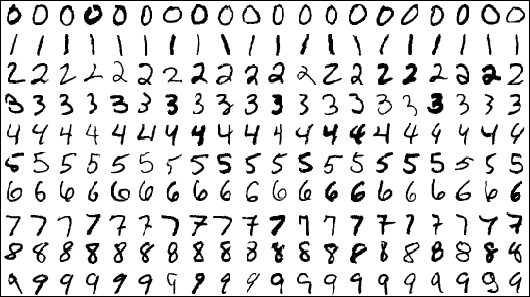
\includegraphics[scale=0.5]{./figures/497Proj_mnist}
\caption{MNIST}
\end{figure}
\item {\bf CIFAR10}\footnote{\url{https://www.cs.toronto.edu/~kriz/cifar.html}} is a datasets consists of $60,000$ color images in $10$ classes, with $6,000$ images per class. There are $50,000$ training data and $10,000$ testing data. Since there are colored pictures, there are three channels, red, green and blue, of the input data. The size is $32\times 32$ pixels for each. It's a subclass of CIFAR100.
\begin{figure}
\centering
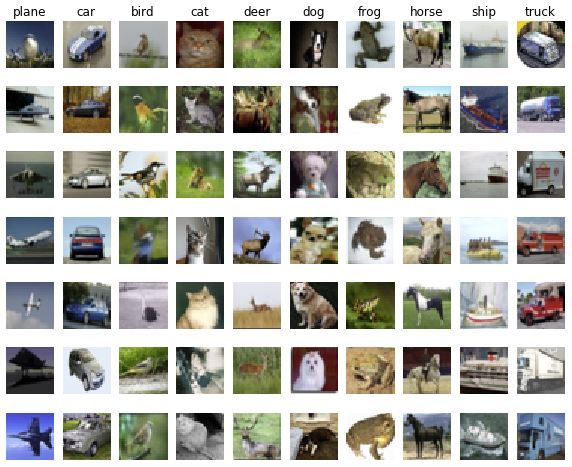
\includegraphics[scale=0.5]{./figures/497Proj_cifar10}
\caption{CIFAR10}
\end{figure}
\item {\bf ImageNet}\footnote{\url{http://www.image-net.org}} is a much larger dataset containing 1.2 millions pictures. The size is $224\times 224$ pixels. The size is much bigger and the quantity is also much larger. So you may get a good performance with a simple neural network on MNIST or CIFAR10, but it's much hard to get good accuracy on ImageNet. %So that why we need   some optimization algorithms on such large datasets.
\begin{figure}[H]
\centering

\includegraphics[scale=0.4]{./figures/497Proj_imagenet}
\caption{ImageNet}
\end{figure}
\end{itemize}
These are three common used datasets that we will use to train our neural networks. 

\subsection{Train an image classifier}
Now we move to a brief PyTorch \footnote{see a quick tutorial \url{https://pytorch.org/tutorials/beginner/deep_learning_60min_blitz.html}} tutorial. To train your first image classifier, these are basically five steps in order:
\begin{enumerate}
\item Load and normalizing the CIFAR10 training and test datasets using torchvision (Here we use CIFAR10 as an example).
\item Define a Convolutional Neural Network. (You can also use a Deep Neural Networks or Recurrent Neural Networks whichever you like.)
\item Define a loss function. (As we just defined before as the function $f$ that is the sum of the total losses.) 
\item Train the network on the training data. (Given the loss function and training data, we can do the steepest descent, stochastic gradient descent or some other optimization algorithms to decrease the loss function on the training set.)
\item Test the network on the test data. (After you have got a good model on your neural network from the last step, then you test your neural network on the test set to see how well it performs. So the final criterion that judges your neural network is the test accuracy because the test set doesn't involve the training process. So it is very important to get a good test accuracy.)
\end{enumerate}
These are all the steps you need to train a neural network. Now let start from the first step.

\subsubsection{Load a dataset}
To load the dataset, we need the libraries, like torch and some others. So we need to import the libraries first.
\begin{python}
import torch
import torchvision
import torchvision.transforms as transforms
\end{python}
This is the first step for all the other codes. And then here is some preprocess of the dataset. Because pictures can be various, you need to preprocess and normalize the pictures to make them have better properties, like the zero mean and small variance, for better interpretation.
\begin{python}
transform = transforms.Compose(
    [transforms.ToTensor(), # Transform the picture to the torch tensor
     transforms.Normalize((0.5, 0.5, 0.5), (0.5, 0.5, 0.5))]) # and then normalize it
\end{python}
Then we define a training set using the \emph{`CIFAR10'} function since CIFAR10 is a default dataset in PyTorch.  The \emph{`root'} is the folder to which we want to store the data. Since we are using the training set, set \emph{`train'} is true. And because we haven't download it before, set \emph{`download'} is true. \emph{`transform=transform'} means we want to transform these pictures following the \emph{`transform'} function that we defined in the preprocess part.
\begin{python}
trainset = torchvision.datasets.CIFAR10(root='./data', train=True, download=True, transform=transform)
\end{python}
Now we have already defined our training set. But there are still some problems. The dataset is too large to load them all to compute the gradient on the full batch. That is why we choose the stochastic gradient descent. So we choose a small batch (mini-batch) to calculate the corresponding gradient. Here we set the batch size to be 4. So we can compute the loss and the gradient very conveniently on each step.  
\begin{python}
trainloader = torch.utils.data.DataLoader(trainset, batch_size=4, shuffle=True, num_workers=2)
\end{python}
It is the same for the test set except that the \emph{`train'} and \emph{`shuffle'} are false. 
\begin{python}
testset = torchvision.datasets.CIFAR10(root='./data', train=False,download=True, transform=transform)
testloader = torch.utils.data.DataLoader(testset, batch_size=4,shuffle=False, num_workers=2)
\end{python}

Here are just some parts to show the images. If you are interested about what the images look like, you can use the \emph{`matplotlib'} library to plot them. If not, just skip this part.
\begin{python}
import matplotlib.pyplot as plt
import numpy as np

# functions to show an image

def imshow(img):
    img = img / 2 + 0.5     # unnormalize
    npimg = img.numpy()
    plt.imshow(np.transpose(npimg, (1, 2, 0)))
    plt.show()

# get some random training images
dataiter = iter(trainloader)
images, labels = dataiter.next()

# show images
imshow(torchvision.utils.make_grid(images))
# print labels
print(' '.join('%5s' % classes[labels[j]] for j in range(4)))
\end{python}

That's basically how you load a dataset. Let's go to the second step.
\subsubsection{Define a Convolution Neural Network}
Since we are dealing with the image classification, we prefer to using the Convolution Neural Network. And we will introduce more details the part later. Now we just go through the codes for the simple example line by line.
The first part is to initialize the class. Then we define how we compute a forward process by given an input as \emph{`x'} in second part.  First, the input will be convoluted with the 2-d convolution operation, then use the ReLU function as the nonlinear activation function, after that we make a pooling. This is what a convolution layer composed, first a convolution operator, then a nonlinear activation, and then a pooling. We define two convolution layers this way.  After that, the function \emph{`x.view'} is used to flat the picture, because the output of the convolution layer is still a two dimensional picture. Here, we use the \emph{`view'} function to flat the two dimensional picture to be one dimensional of length 400. Then we make a fully connect operator and a ReLU function. After that, we have the final classification layer to output the prediction outcome. So that is basically what the CNN composed.
\begin{python}
import torch.nn as nn
import torch.nn.functional as F

class Net(nn.Module):
    def __init__(self):  # Initialize the class
        super(Net, self).__init__()
        # the construction of the neural network
        self.conv1 = nn.Conv2d(3, 6, 5) # a 2-d convolution layer named as `conv1'
        self.pool = nn.MaxPool2d(2, 2) # a max pooling layer named `pool'
        self.conv2 = nn.Conv2d(6, 16, 5)
        self.fc1 = nn.Linear(16 * 5 * 5, 120) # linear layer
        self.fc2 = nn.Linear(120, 84)
        self.fc3 = nn.Linear(84, 10)

    def forward(self, x):  
        x = self.pool(F.relu(self.conv1(x))) 
        x = self.pool(F.relu(self.conv2(x))) 
        x = x.view(-1, 16 * 5 * 5)
        x = F.relu(self.fc1(x))
        x = F.relu(self.fc2(x))
        x = self.fc3(x)
        return x


net = Net()
\end{python}
Different choices of these hyper-parameters may lead to different results. We usually need to tune these hyper-parameters to get a better model. 
Since the input of each layer in the neural network is the output of its previous layer, there are two parts of hyper-parameters of an operator, like \emph{`Conv2d'}, \emph{`Linear'}. One part depends on the input, which is the output of the previous layer, of this operator. The other can be arbitrarily choose to get a good model, and this part may decide a part of parameter of the next operator/layer. For example, `Linear(input dimension, output dimension)', the dimension of output of \emph{`fc1'} is 120, then the first parameter of \emph{`fc2'} should be same as it, 120.  

Another important hyper-parameters of convolution layers is channel. For \emph{`Conv2d (number of input channels, number of output channels, kernel size)'}, we need keep the number of input channel same as the number of output channel of the previous layer.   

To choose parameters (called hyper-parameters in neural network) of the torch functions, we recommend to read the corresponding documents in PyTorch website for more precise details.

Here we just give a simple working example. Later on, we will talk about more details and how to modify them.

\subsubsection{Define a loss function and optimization}
There are actually a lot of possible loss functions. For image classification, the common choice is the cross-entropy. You can also use the square loss or any reasonable functions based on the problems. Actually, the common loss functions have already been defined in the \emph{`torch.nn'} library. The way to use them is like the \emph{`criterion'} in the following code. And the \emph{`optimizer'} is the corresponding optimization algorithm used to decrease the loss function. The common algorithms can also be found in the \emph{`torch.optim'} library. In the example, we choose stochastic gradient descent (SGD). And there are a few optional parameters, like learning rate \emph{`lr'}, momentum. For large learning rate, you may behave very widely, but for small learning rate, you may zig-zaging around very small range. The learning rate is one of the most important hyper-parameter that we need to tune to get a good model.
\begin{python}
import torch.optim as optim

criterion = nn.CrossEntropyLoss() #use the cross-entropy loss defined in torch library
optimizer = optim.SGD(net.parameters(), lr=0.001, momentum=0.9)
\end{python}     

Now we have almost defined everything. Then we can start to train our networks. 
\subsubsection{Train the network}
For the training, we first define what the epoch means. Because we have like 60,000 pictures in this training set, and we divided it into a few small batches (mini-batch). Whenever you go over all the pictures in the training set, then it means you finish an epoch.
And when we do one optimization step (calculate gradient and update the parameters) in one mini-batch, we say it an iteration.
\begin{python}
for epoch in range(2):  # loop over the dataset multiple times

    running_loss = 0.0 
    for i, data in enumerate(trainloader, 0): # i is the index and data are pictures in the corresponding mini-batch
        # get the inputs; data is a list of [inputs, labels]
        inputs, labels = data

        # zero the parameter gradients
        optimizer.zero_grad()

        # forward + backward + optimize
        outputs = net(inputs) # forward propagation to get the output
        loss = criterion(outputs, labels) # compute the loss, see if it satisfy the terminal criterion
        loss.backward() # backward propagation to get the gradient
        optimizer.step() # update the parameters by optimization algorithm (like SGD) to decrease the loss

        # print statistics
        running_loss += loss.item()
        if i % 2000 == 1999:    # print every 2000 mini-batches
            print('[%d, %5d] loss: %.3f' %
                  (epoch + 1, i + 1, running_loss / 2000))
            running_loss = 0.0

print('Finished Training') # After 2 epochs, we finish the training.
\end{python}

Now, after training process, we want to see how well the model behave. So let's start to test the model we got on the test set, which is independent to the training.
\subsubsection{Test the network on the test data}
\begin{python}
correct = 0 
total = 0
with torch.no_grad(): # We don't need compute the gradients in the test process since we don't need optimization
    for data in testloader:
        images, labels = data
        outputs = net(images)
        _, predicted = torch.max(outputs.data, 1) # get the predicted class by neural network
        total += labels.size(0)
        correct += (predicted == labels).sum().item() # compare the predicted and the real label

print('Accuracy of the network on the 10000 test images: %d %%' % (100 * correct / total))
\end{python}
Now we finish training a simple neural network here.



